\section{PO advice for next the next year PO group} \label{appendix:PO-advise}

This document servers as a list of advice for the next PO group based on the experience we gathered throughout the semester.
\\
The PO group's main responsibility is to communicate with the customers of the GIRAF project and document this interaction.
It is important that the customers reactions, opinions and wishes, towards the program, are written down as these are the base for all the decisions that you as the PO group will take.
Further in-depth of how we advise to handle customer contact and what we used the information gathered is described in the following sections.

\subsection{Customer contact}
In the start of the semester Ulrik will most likely schedule some meetings with the customers which everyone should attend to get up to speed with what exactly the GIRAF project is and how the program is supposed to help people diagnosed with autism.
Already before these meetings it is a good idea to contact the customers to try and arrange time for a more secluded meeting where you as the PO group can ask more specific questions about how they want the program to function and the design to look.
The other groups should not be present for these meetings as it is your responsibility to relay this information to the other groups.
We arranged a meeting with Emil from Egebakken right after his presentation. 
A transcription of this interview can be seen in \autoref{appendix:trans-emil}.
It is a very good idea to get there phone numbers if possible as it has been evident that communication through mail often is very lacking.
\\
After this you should have a good idea of what the customers want and you can start setting goals for what should be completed in the upcoming sprint as well as for the whole semester.
\\
As soon as you have the dates for you sprints you should contact as many customers as you can with dates for usability testing, we did this by sending a mail to every customer involved in the project.
Remember to schedule usability testing after your releases so that you have a working program for the customers to test and evaluate.
It is important that you ask the customers to confirm that they will participate in these test.
If they do not respond you should try and contact them to see if they simply forgot to reply, this was often done by calling them on their phones or by calling their workplaces.
\\
To reiterate, it is very important to take notes and document all meetings with customers.
There is going to be a lot of questions by developer groups about how functionality should be made and how it should look.
Therefore it is always better to have written down exactly what the customers want so that you do not have to guess and then refactor later when you guessed wrong.
An issue we faced was that we thought it would be sufficient for a guardian to copy activities one day at the time, but when we showed prototypes to the guardians they were very adamant on having the functionality to copy to multiple days at once.
\\
Another reason to document as much as possible is that the users feedback is the basis of all the user stories you are going to create.
It is also important that your user stories are not written ambiguous and if so that you have the precise functionality that the users wanted.

\subsection{Creating user stories}
As the PO group it is your responsibility to create user stories.
User stories are created based on requests from the users.
We structured user stories in the following way:
\begin{itemize}
    \item As a ... I would like ..., so that ...
\end{itemize}

When creating user stories you should consider the amount of work that is needed for it to be completed and whether it should be split up into multiple smaller user stories.
We created user stories in the weekplanner repository on our GitHub page under the issue tab.
This made it easy to organize as user stories are uniquely numbered and can be put into milestones.
When creating a pull request it is then easy to tag the user story so that it will be automatically closed when the pull request has been merged.
It also allowed us to assign them with tags such as "feature" and give them different priorities ranging from lowest to highest.
A user story should if needed contain a prototype that optimally has been approved by a customer and a further description of the problem.
We also had great success having one of the more experienced flutter developers write a short comment explaining how they would structure the solution for the user story.
This gave the developers who was not as experienced with flutter a better starting point.
\\
Below is an image of a user story.
\begin{figure}[h]
    \centering
    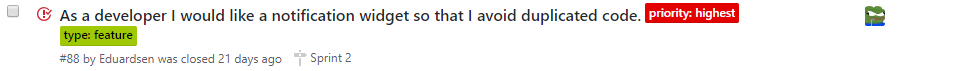
\includegraphics[width=1.0\textwidth]{userStory.PNG}
    \caption{User story \#88 from sprint 2}
    \label{fig:userstory}
\end{figure}
As you can see on \autoref{fig:userstory} the user story has the number 88 and was created by the user Eduardsen.
It has the tags "priority: highest" and "type: feature" and is under the milestone called sprint 2.
In the right hand side you can see the profile picture of the user currently assigned to fixing this user story.

\subsection{Prototypes}
One of the important tasks of the PO group is to create and maintain prototypes.
Prototypes should conform to the design guide which can be found on the Github Wiki-page.




What is the role of the PO group? -----
Customer contact----
Creating user stories ----
prototypes
distribution of tasks
Communication with other groups (keeping status)
-Making sure that groups dont work on the same files more than necessary
Approval of designs
release preperation
usability testing
maintenance of user stories
Approval of bug reports
cooperation with the process group
planning of sprints
be present in your group rooms so that people can ask you questions
sharing knowledge in the po group




for





